\documentclass[a4paper,10pt]{article}
%\usepackage[latin1]{inputenc} % Paquetes de idioma
\usepackage[utf8]{inputenc} % Paquetes de idioma (Este encoding toma acentos :) )
\usepackage[spanish]{babel} % Paquetes de idioma
\usepackage{graphicx} % Paquete para ingresar gráficos
\usepackage{grffile}
\usepackage{hyperref}
\usepackage{fancybox}
\usepackage{amsmath}
\usepackage{amsfonts}
\usepackage{listings}
\usepackage{float}
% Paquetes de macros de Circuitos
%\usepackage{pstricks}
\usepackage{tikz}

% Encabezado y Pié de página
\usepackage{fancyhdr} % Paquete para encabezados y pie de página
\pagestyle{fancy} % Sin esta línea no se imprimiría el encabezado en todas las páginas

\fancyhf{} %  Borra el encabezado anterior (Por defecto escribe el títutlo de la sección en la que se encuentra la hoja
\setlength{\headheight}{22.55pt}
\fancyhead[L]{
	{\textsf{Facultad de Ingenier\'ia $-$ Universidad de Buenos Aires \\ 66.44 Instrumentos Electrónicos}}
}
%\addtocounter{page}{5}
\fancyhead[R]{\thepage}

\renewcommand{\footrulewidth}{0.4pt} % Ajusta el tamaño de las líneas separadoras en el pié de página
\renewcommand{\headrulewidth}{0.4pt} % Ajusta el tamaño de las líneas separadoras en el encabezado

\fancyfoot[L]{
	{\textsf{Trabajo Pr\'actico N$^{\circ}4$}: Mediciones de impedancias} \\
	{\textsf{Integrantes: Eduardo Sanchez, Francisco Soler}}
	}
		

% Carátula del Trabajo
\title{ \author{} % Lo pongo para que el warning no moleste :p
\setlength{\unitlength}{1cm} %  Especifica la unidad de trabajo
\thispagestyle{empty}

\begin{picture}(18,0)
\put(0,0){
\includegraphics[width=1.5cm, height=3cm]{Logo1.png}}

\put(10.5,0){
\includegraphics[width=3cm, height=3cm]{Logo2.png}}

\end{picture}
\\[1.5cm]
\begin{center}
	\textbf{{\Huge Facultad de Ingenier\'ia \\ Universidad de Buenos Aires}}\\[2cm]
	{66.44 Instrumentos Electrónicos}\\[0.5cm]
	{Trabajo Pr\'actico N$^{\circ}3$: Mediciones de impedancias}\\[2.5cm]
\end{center}

\begin{flushleft}
	\textbf{Integrantes:} \\[1cm]

	\begin{tabular}{|c|c|c|}
		\hline
		\textbf{\normalsize Padr\'on} & \textbf{\normalsize Nombre} & \textbf{\normalsize Email} \\
		\hline
		\normalsize 92903 & \normalsize Sanchez, Eduardo Hugo & \normalsize hugo\_044@hotmail.com \\
		\hline
		\normalsize 91227 & \normalsize Soler, Jos\'e Francisco & \normalsize francisco.\_tw@hotmail.com \\
		\hline
		\normalsize xxx & \normalsize Wawrynczak, Claudio  & \normalsize claudiozak@gmail.com \\
		\hline
	\end{tabular}
\end{flushleft}
\date{} % Hace que no se imprima la fecha en la cual se compilo el .tex
 }

\begin{document}
	\maketitle % Hace que el título anterior sea el principal del documento
	\newpage

	\tableofcontents % Esta línea genera un indice a partir de las secciones y subsecciones creadas en el documento
	\newpage


	\section{Objetivo}
	
	\indent	El objetivo del presente trabajo práctico es determinar el comportamiento y fiabilidad de 3 tipos de puntas de medición, de tensión con alta/baja impedancia de entrada, y de corriente.
	
	\newpage
	\section{Desarrollo}
		\indent Para llevar a cabo las mediciones, se utilizan los siguientes instrumentos:
		\begin{itemize}
			\item Un generador de señales con la capacidad de realizar un barrido en frecuencias.
			\item Un osciloscopio con la capacidad de cambiar a alta o baja su impedancia de entrada.
			\item Las puntas de prueba.
			\item Un cable que interconecta el generador con el osciloscopio, el cual, se comporta como una línea de transmisión.
		\end{itemize}
				 
		\subsection{Punta de prueba de alta impedancia}
		Se conecta el generador de se\~nales a la entrada del CH1 del osciloscopio cuya impedancia de entrada es de $50 \Omega$, al igual que la impedancia caracter\'istica del cable coaxil que los conecta, de manera que exista adaptaci\'on. Por otra parte al CH2 del osciloscopio se conecta una punta X10, la cual sensa la tensi\'on a la entrada del CH1.
		El generador de se\~nales realiza un barrido de frecuencias de $1MHz$ a $400MHz$ en $10s$
		En la Figura \ref{img001} se puede observar las se\~nales que recibe el CH1 cuando est\'a conectado al generador de funciones (la cual se guarda como referencia) y la que recibe cuando adem\'as se carga el nodo del CH1 con la punta que se conecta al CH2.
			\begin{figure}[!htb]
				\centering
				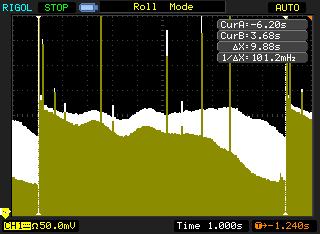
\includegraphics[width=8cm]{Imagenes/Mediciones instrumentos/NewFile1.png}
				\caption{Se\~ales recibidas en CH1 cuando est\'a conectado al generador de se\~ales (en blanco) y cu\'ando se carga con la punta X10 (en verde)} \label{img001}
			\end{figure}
		Como era de esperar al cargar el nodo con la punta X10, el ancho de banda disminuye considerablemente.
		En la Figura \ref{img000}
			\begin{figure}[!htb]
				\centering
				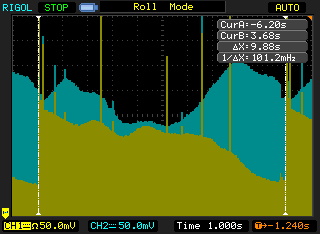
\includegraphics[width=8cm]{Imagenes/Mediciones instrumentos/NewFile0.png}
				\caption{Esquemático de IPSec en modo t\'unel} \label{img000}
			\end{figure}
			
			\begin{figure}[!htb]
				\centering
				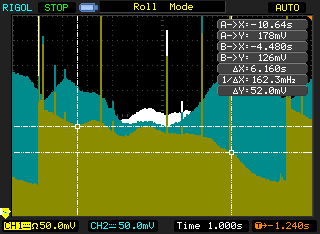
\includegraphics[width=8cm]{Imagenes/Mediciones instrumentos/NewFile2.png}
				\caption{Esquemático de IPSec en modo t\'unel} \label{img003}
			\end{figure}						
		\subsection{Punta de prueba de baja impedancia}
		\subsection{Punta de prueba de corriente}
		
		
	


	
		
\end{document}

